\subsection{Алгоритмы трассировки лучей}
Суть метода заключается в отслеживании траекторий лучей и расчета взаимодействий с лежащими на траекториях объектами, от момента испускания лучей источником света до момента попадания в камеру. Под взаимодействием луча с объектами понимаются процессы диффузного (в смысле модели локальной освещенности), многократного зеркального отражения от их поверхности и прохождение лучей сквозь прозрачные объекты. Таким образом, ray tracing – первый метод расчета глобального освещения, рассматривающий освещение, затенение (расчет тени), многократные отражения и преломления. Различают два основных вида метода трассировки лучей: \textbf{\textit{прямой}} -- \index{forward ray tracing}forward ray tracing, и \textbf{\textit{обратный}} -- \index{backward ray tracing}backward ray tracing.

\subsubsection{Прямой метод трассировки лучей}
В прямом методе траектории лучей строятся от источника ко всем точкам всех объектов сцены (первичные лучи). Затем проверяется ориентация каждой точки относительно источника, и, если она лежит на стороне объекта, обращенной в противоположную от источника сторону, точка из расчетов освещенности исключается. Для всех остальных точек вычисляется освещенность с помощью локальной модели освещения. Если объект не является отражающим или прозрачным, то есть поверхность объекта только диффузно рассеивает свет, траектория луча на этой точке обрывается (заканчивается). Если же поверхность объекта обладает свойством отражения (\index{reflection}reflection) и/или преломления (\index{refraction}refraction), из точки строятся новые лучи, направления которых совершенно точно определяются законами отражения и преломления.
\par
    Для построенных таким образом траекторий новых лучей может быть только три исхода. Луч либо выходит за пределы видимой из камеры области сцены, в этом случае все проделанные для него до этого момента расчеты освещенности отбрасываются, поскольку они не принимают участия в формировании изображения. Или луч попадает в камеру, тогда рассчитанная освещенность формирует цвет соответствующего пиксела изображения. Или луч встречает на своем пути новый
объект, тогда для новой точки пересечения повторяется расчет освещенности и построения лучей отражения и преломления в зависимости от свойств поверхности объекта (рекурсия). Построение новых траекторий и расчеты ведутся до тех пор, пока все лучи либо попадут в камеру, либо выйдут за пределы видимой области. Очевидно, что при прямой трассировке лучей мы вынуждены выполнять расчеты для лучей, которые не попадут в камеру, то есть, проделывать бесполезную работу. По некоторым оценочным данным доля таких "слепых"лучей довольно велика. Эта главная, хотя и далеко не единственная, причина того, что метод прямой трассировки лучей считается неэффективным и на практике не используется(в чистом виде).

\subsubsection{Обратный метод трассировки лучей}
Обратной метод трассировки лучей, или backward ray tracing. Этот метод расчетов основывается на построении лучей от наблюдателя через плоскость экрана вглубь сцены, а не от источника, то есть -- наоборот. Этот способ достаточно изящен, что позволяет решить массу проблем, возникающих при прямой трассировке, а сам метод отличается простотой и понятностью. Лучи теперь строятся иначе. А именно, по двум точкам: первая точка, общая для всех лучей – положение камеры (наблюдателя), вторая точка определяется положением пиксела на плоскости видового окна. Таким образом, направление каждого луча строго определено (две точки в пространстве определяют одну и только одну прямую – школьный курс геометрии), и количество первичных лучей также известно – это общее количество пикселей видового окна. Например, если видовое окно имеет 1920 пикселей по ширине и 1200 пикселей по высоте, количество лучей составит 1920 х 1200 = 2 304 000. Каждый луч
вдоль заданного направления продлевается от наблюдателя вглубь трехмерной сцены, и для каждой траектории выполняется проверка на пересечение со всеми объектами сцены и с отсекающими плоскостями. Если пересечений с объектами нет, а есть пересечение только с плоскостью отсечения, значит луч выходит за пределы видимой части сцены, и соответствующему пикселю видового окна присваивается цвет фона. Если луч пересекается с объектами сцены, то среди всех объектов выбирается тот, который ближе всего к наблюдателю. В точке пересечения с таким объектом строится три новых, так называемых вторичных луча. \par

\begin{center}
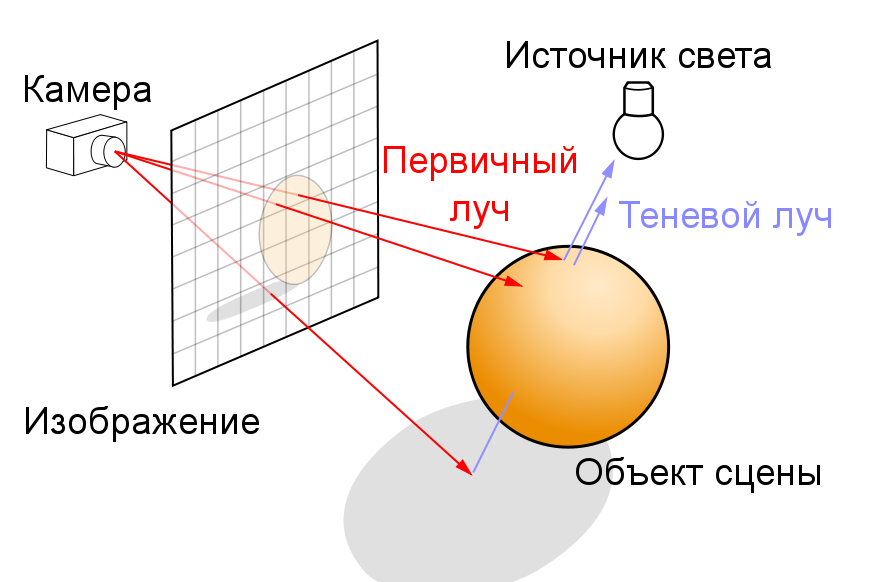
\includegraphics[scale=0.5]{imgs/Ray_trace_diagram_rus.png} 
\end{center}

Первый луч строится в направлении источника света. Если источников несколько, строится несколько таких лучей, по одному на каждый источник. Основное назначение этого луча – определить ориентацию точки (обращена точка к источнику или от него), наличие объектов, закрывающих точку от источника света, и расстояние до источника света. Если точка обращена в противоположную сторону от источника света или закрыта другим непрозрачным объектом, освещенность от такого источника не рассчитывается, точка находится в тени. В случае затеняющего прозрачного объекта интенсивность освещения уменьшается в соответствии со степенью прозрачности. Если точка закрыта от освещения всеми источниками сцены, ей присваивается фоновый (\index{ambient или фоновый цвет}ambient) цвет. В противном случае точка освещена, интенсивность и цвет освещения рассчитываются при помощи локальной модели освещенности, как сумма освещенностей от всех источников, для которых эта точка не закрыта другими объектами. Этот тип луча получил название \index{shadow ray или теневой луч} \textit{\textbf{shadow ray}} (иногда его еще называют \index{illumination ray}illumination ray) – теневой луч. Если поверхность объекта не является отражающей и непрозрачна, теневой луч – единственный тип лучей который строится, траектория первичного луча обрывается (заканчивается), и дальнейшие расчеты не выполняются. Рассчитанный цвет (освещенности или тени) присваивается тому пикселю видового окна, через который проходит соответствующий первичный луч.
   \par
   Второй луч строится, если поверхность объекта обладает отражающими свойствами, и называется \index{reflection ray или отраженный луч} reflection ray, или луч отражения. Направление отраженного луча определяется по закону:
$$
	\vec{R} = \vec{I} - 2 \cdot \vec{N} (\vec{N} , \vec{I})
$$
где $\vec{R}$ - отраженный луч, $\vec{I}$ - падающий пераичный луч, $\vec{N}$ - нормаль к поверхности в точке соударения.
Для отраженного луча проверяется возможность пересечения с другими объектами сцены. Если пересечений нет, то интенсивность и цвет отраженного луча равна интенсивности и цвету фона. Если пересечение есть, то в новой точке снова строится три типа лучей – теневые, отражения и преломления.
Третий луч строится, если поверхность объекта прозрачна, и носит название \index{transparency ray или преломленный луч}transparency ray, т. е. луч преломленный. Направление для преломленного луча определяется следующим образом:
$$
 \vec{T} = \frac{n_1}{n_2} \cdot \vec{I} - \left[ \cos \alpha + \frac{n_1}{n_2} \cdot \left(\vec{N},\vec{I} \ \right) \right] \cdot \vec{N}
$$
$$
\cos \alpha = \sqrt{1 - \left( \frac{n_1}{n_2} \right) ^2 \cdot \left(1-\left(\vec{N},\vec{I}\ \right)^2\right)}
$$
где $\vec{T}$ - переломленный луч, $n_1$ - коэффициент рефракции для первой среды ( в которой растространяется первичный луч ), $n_2$ - коэффициент рефракции для второй среды прозрачного объекта.

Так же, как и в предыдущем случае, проверяется пересечение вновь построенного луча с объектами, и, если они есть, в новой точке строятся три луча, если нет -- используется интенсивность и цвет фона.

Таким образом, для каждого первичного луча можно построить древовидную структуру. Если древовидная структура для данного луча построена, то расчет освещенности можно выполнить в следующем порядке. Для каждой ветви дерева спускаемся вдоль древовидной структуры к последнему пересечению вторичного луча и поверхности (будем дальше называть их узлами). Поскольку это последний узел в цепи, то  вкладов от преломлений и отражений нет, поэтому, освещенность узла вычисляется при помощи локальной модели освещения с учетом видимости источников света для данного узла. Затем, вычисленная освещенность передается вверх по ветви к следующему ближайшему узлу. Освещенность в этом узле будет вычисляться по формуле:

$$
 \vec{I}_{total} = \vec{I}_{local} + K_{reflection} \cdot \vec{I}_{reflection} + K_{refraction} \cdot \vec{I}_{refraction}
$$

где $\vec{I}_{total}$ - полная освещенность в точке, $\vec{I}_{local}$ - локальная освещенность в точке, вычисленная от источников освещения с помощью одной из локальной модели освещенности, $K_{reflection}$ - коэффициент, определяющий отражающие свойства поверхности, $\vec{I}_{reflection}$ - освещенность предыдущей точки, переданная вдоль ветки отражения,   $K_{refraction}$ - коэффициент, определяющий преломляющие свойства поверхности $\vec{I}_{refraction}$ - освещенность предыдущей точки, переданная вдоль ветки преломления

Естественным завершением трассировки лучей является выход всех испущенных вторичных лучей за пределы видимой области и их рассеяние на чисто диффузных объектах. Результат вычислений будет наиболее точным. Но, если сцена достаточно сложна, такой расчет будет очень медленным, а в некоторых случаях и невозможным по причине ограниченности аппаратных ресурсов. Легко увидеть, что вклад освещенности от каждого нового вторичного луча очень быстро уменьшается по той простой причине, что коэффициенты свойств отражения и преломления материалов меньше единицы. Поэтому часто трассировку лучей прекращают, когда вклад от следующего узла ветви становится меньше заданной величины. Это также достаточно точный метод расчетов, который может быть использован для получения качественных результатов при определенных условиях. Наконец, для получения оценочного расчета можно оборвать трассировку лучей после выполнения заданного количества итераций, это самый быстрый и наименее точный расчет.

\subsubsection{Достоинства и недостатки}

Основные достоинства рекурсивного метода обратной трассировки лучей – расчет теней, многократных отражений и преломлений, значительно повысивших степень реалистичности получаемых изображений.
Основные недостатки: неучет вторичного освещения от диффузно отраженного объектами света; низкая скорость и высокая вычислительная стоимость расчетов – в классическом рейтресинге необходимо проверять на пересечение каждый луч со всеми объектами сцены, в результате от 70 до 95 процентов всего времени расчетов тратится на вычисление пересечений; резкие границы цветовых переходов тени/подсветок/прозрачности; \index{aliasing}aliasing – "зазубренность" линий и т. д.; дискретность определяющих цвет пиксела первичных лучей – одного первичного луча недостаточно для корректного определения цвета пиксела, формирующего изображение.
